% ============================
% TP Report – Simple Two-Column Template
% ============================
\documentclass[10pt,a4paper,twocolumn]{article}

% ---- Encoding & typography (simple, portable) ----
\usepackage[utf8]{inputenc}
\usepackage[T1]{fontenc}
\usepackage{lmodern}
\usepackage{microtype}

% ---- Layout ----
\usepackage{geometry}
\geometry{
  left=1.5cm, right=1.5cm,
  top=1.6cm, bottom=1.6cm,
  columnsep=0.6cm
}
\usepackage{balance} % balances the final page columns

% ---- Graphics ----
\usepackage{graphicx}
\usepackage[font=small,labelfont=bf]{caption}

% ---- Useful tweaks (optional) ----
\setlength{\parskip}{0pt}   % compact paragraphs
\setlength{\parindent}{1em} % classic indent; comment out if you prefer no indents

% ============================
%            Title
% ============================
\title{\vspace{-6mm}\textbf{TP Report Title: Short and Informative}}
\author{BONDIL Maxime - DE BACKER Mathis \quad G1 Polytech \\ Instructor: Mahdi Khoramshahi }
\date{\today}

\begin{document}
\maketitle

% ============================
%         One-sentence intro
% ============================
% Keep this to 2–3 lines max; no abstract section to stay minimal.
\noindent\textbf{Context.}Dans ce TP nous avons tester des situations où l'on peut découplé les équation et annuler certian inconnues des équations nous permettant d'isolé et d'identifier un plus petit groupe d'inconnues, pour ensuites identidier les plus complexes. 


% ============================
%           Sections
% ============================
\section*{Problem Statement}
Les inconnues des equations du sytème cromprennent les termes d'inertie, centrifuges, de gravité et de frottements, en plus de ça les deux equations du systeme sont couplé dans un sens car le mouvement du premier moteur engendre une rotation du deuxieme.\\
On cherche ensuite à traiter chaque moteur séparement. On établie des situations où les deux moteurs sont découplé, ce qui nous donne : les terme d'inertie et centrifuge son nul, les termes de gravité sont decouplé. Pour ainsi pouvoir identifié les parametres gravitaires et de frottements restant.\\
Grace aux parametres trouvé on peut maintenant isloer et determiner les parametres manquant d'inertie et ceux centrifuges.

\section*{Method and Implementation}
On a fait attention a ce que le nombre "n" de donné (q1, q2, qp1, qp2 ...) soit bien dimensionné en fonctioons des parametres que l'on étudie en utilisant : n = size(q1).
Comme pour le TP1 on a fait deux matrice (A et u) qui s'ajuste en fonction du nombre de données.
En utilisant la formule du cours on peut verifie que les parametres trouvés on la meme echelle d'erreur.

% ============================
%     Main Results Figure
% ============================
% Use figure* to span both columns. Replace results.pdf with your image file.
\begin{figure}[!h]
  \centering
  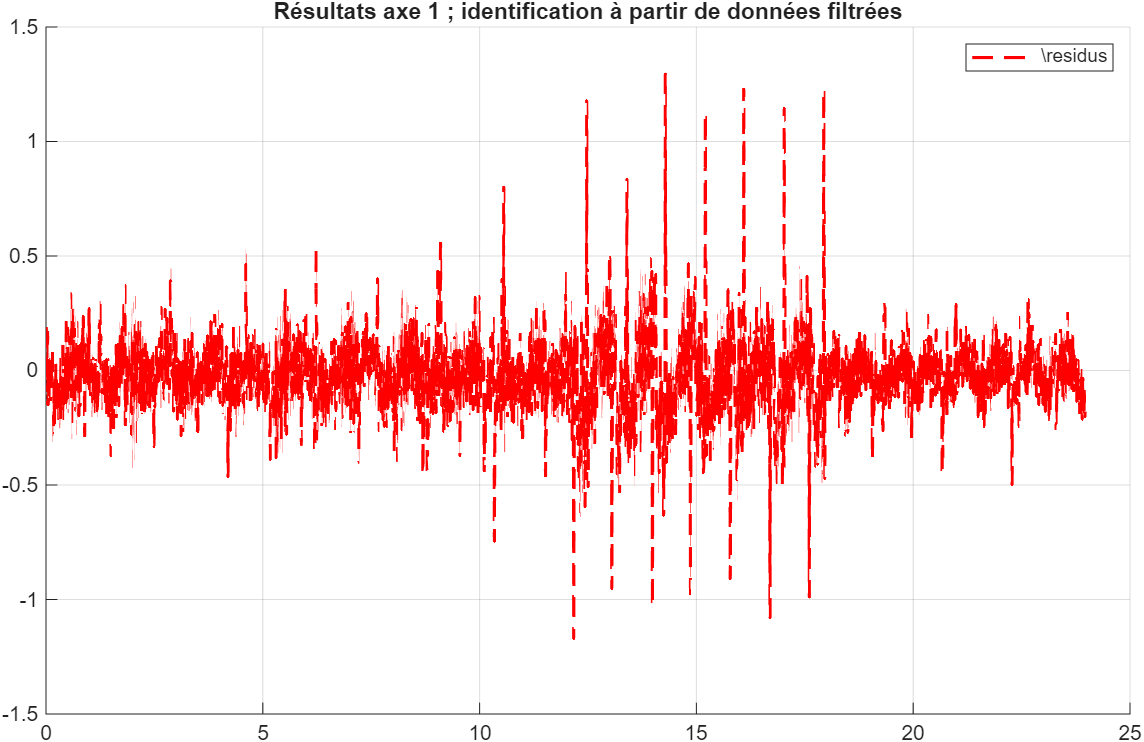
\includegraphics[width=0.45\textwidth]{fig_parameters.png}
  \caption{Résultats axe 1 ; identification à partir de données filtrées}
  \label{fig:summary}
\end{figure}

\section*{Results}
On observe que les parametre filtré nous donne une valeur assez proches ou la meme suivant les parametres de ce non filtrés mais on ne sait pas les plus veridicte, même si on va supposé que ceux filtré sont plus exactes.\\
On observe sur le graphique \ref{fig:summary} que la difference entre le signal de sortie trouvée et réel ressemble a une sinuzoide très bruité qui correspond à l'élément que l'on n'a pas pris en compte lors de notre etude : la courroie.

\section*{Conclusion}
On a aprris qu'il fallait trouvé découplé notre systeme pour pouvoir identifier les parametre de celui-ci, et ne pas hesiter a essayer d'annuler le plus de terme et au fur et a mesure les rajouter un par un si possible. Il ne faut pas oublié ce qu'on ne modelise pas (comme la courroie) par simplicité a toujours une réercution sur le résultat final.

% Balance last page columns and end.
\balance

\end{document}
